video notes: vid14.mp4
\subsection*{Mininum Phase Filters (Z-plane)}
\begin{itemize}
\item{All poles and zeros inside the unit circle in the z-plane 
OR all in the left-half plane (LHP) in the splane}
\item{Easy to talk about s-plane by replacing the interior of the unit circle by
the left half plane, the "stability region"}

\item{
Trivial Example: one pole one zero lowpass filter (z-plane)
}
\item{
    Adding a zero outside that circle makes it not minum phase
    \paulhint{See diagram taken at 1:56, 23a}
    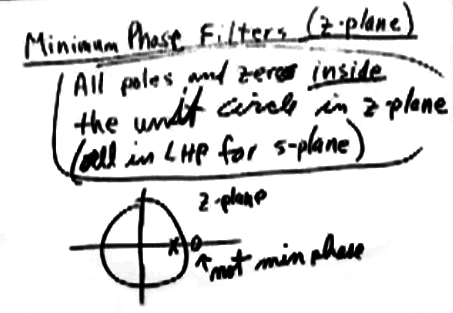
\includegraphics[scale=0.4]{frames/23a}
}
\item{
    To make it MP it needs to be inside the unit circle, (they can't even
touch the unit circle)
}


\item{
Example:  $h(n) = [a, b, 0\cdots]$, $H(z) = a + bz^{-1}$
    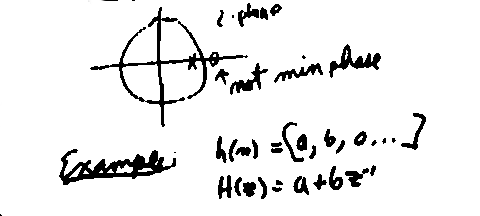
\includegraphics[scale=0.4]{frames/23b}
\paulhint{See diagram taken at 2:46, 23b}

}
\item{
It's a really trivial FIR filter of length 2, first order
}
\item{
Under what conditions is this a minimum phase filter? It's a one
zero filter zero at $q_1 = -b/a$.
}
\item{
$[1, 2]$ is not minimum phase, $[2, 1]$ is. MPF decays: it is a characteristic.
}
\end{itemize}
\subsection*{Allpass fitlers}
\begin{itemize}
\item{
$\vert H(e^{j\omega T}) \vert = 1$ (or any constant, but normally 1 if you can 
get it)
}
\item{
$
\frac{\vert B(e^{j\omega T} \vert}
{\vert A(e^{j\omega T} \vert}
$ or 
$\vert B(e^{j\omega T} \vert =
\vert A(e^{j\omega T} \vert$
}
\item{
Having them be the same is fine, but they will just cancel and you'll get 
a wire (which is technically an allpass, but not an interesting one)
}
\item{
More interesting: let $B = \mbox{Flip}(A)$, ie
$B(z) = z^{-n}A(z^{-1})$
}
\item{ 
To elaborate:
\paulhint{See diagram taken at 7:52, 23c}
    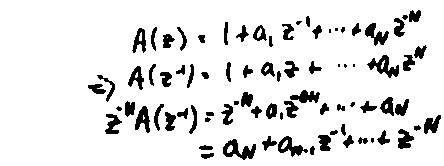
\includegraphics[scale=0.4]{frames/23c}
}
\item{
You are flipping the coefficients without moving the powers of $Z$.
}
\item{
\textbf{Example: order 1}
$H(z) \frac{a_1 + z^{-1}}{1 + a_1 z^{-1}}$\\
$\vert H(e^{-j\omega T}) \vert =
\vert \frac{a_1 + e^{-j \omega T}}{1 + a_1 e^{-j\omega T}}\vert$\\

$\vert H(e^{-j\omega T}) \vert =
\vert 
\frac{a_1 + e^{-j \omega T}}{
e^{j\omega T} + a_1
}
\vert
$\\
$ = \vert \frac{\overline{d}}{d} \vert = 1 
$\\
$\frac{
\vert e^{-j\Theta_d}\cdot r_d \vert
}{
\vert e^{j\Theta_d}\cdot r_d \vert
} = 1$
\paulhint{See diagram taken at 11:25, 23d}
    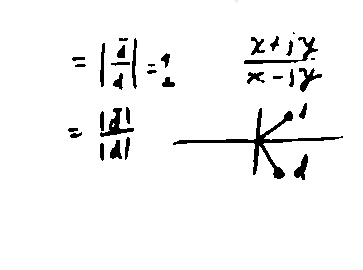
\includegraphics[scale=0.4]{frames/23d}
}
\item{
$A(z^{-1})$ has roots at $\frac{1}{p_i}$ where $A(p_i) = 0$
}
\item{
$A(z^{-1})$ are the locations of our zeros. Because the zeros
are the roots of A, they are at the poles reciprocated.
}
\item{
This inverse is the reciprocol of the magintude and the 
conjugated phase: if it's on the unit circle, it will flip
to the other side. Since poles are in complex conjugate 
pairs, you don't really need to think about the "flip"
}
\paulhint{See diagram taken at 14:13, 23e}
    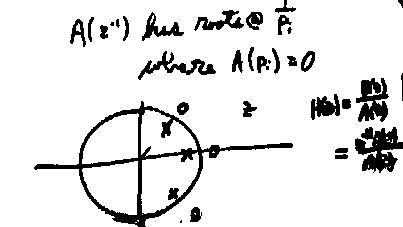
\includegraphics[scale=0.4]{frames/23e}
\item{
\textbf{s-plane allpass}:
The distances from the $j\omega$ axis are the same, but flipped,
it is a left-right flip. How do I express this (inverse doesn't work)?You make $A(s)$ $A(-s)$. 
}
\item{
This flip is a bit of a trick: it is a double flip, it's a left/right AND a up/down flip. Since we assume real coefficients, there is
up/down symmetry. 
\paulhint{See diagram taken at 16:01, 23f}
    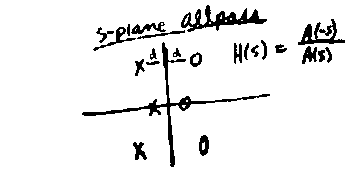
\includegraphics[scale=0.4]{frames/23f}
}
\item{
to make $H(s) = \frac{}{s^2 + \frac{1}{Q}s + 1}$, an all pass, we make s
negative on the numerator:
$H(s) = \frac{s^2 - \frac{1}{Q}s + 1}{s^2 + \frac{1}{Q}s + 1}$
How easy is that?
}
\item{To make an allpass: in the z-plane, we inverse, in the s-plane, we negate (all the odd powers)}
\end{itemize}

\subsection*{Phase of Allpass}
\begin{itemize}
\item{$\angle H$ = $\angle B - \angle A$}
\item{$\angle H$ = $- 2\angle A$, $B = \mbox{Flip}(A)$}
\end{itemize}
\subsection*{Bonus: Phasers constructed from Biquad allpass filters}

\paulhint{See diagram taken at 25:23, 23g}
    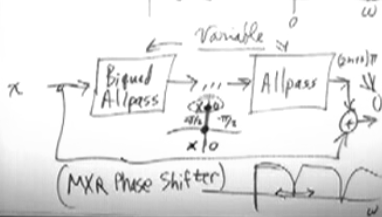
\includegraphics[scale=0.4]{frames/23g}

\subsection*{Allpass and Minimum phase}
\begin{itemize}
\item{Any filter can be expressed as an allpass times a minimum phase
filter}
\item{A non-minimum phase filter has a zero in the RHP. All you do
is decompose that and reflect the zeros, and the all pass you introduce
cancels the zero:
\paulhint{See diagram taken at 27:02, 23h}
    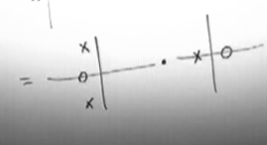
\includegraphics[scale=0.4]{frames/23h}
}
\item{
Minimum phase assumes filter stability.
}
\end{itemize}

